%----------------------------------------------------------------------------------------
%	Section: PRo3D Command Line Interface
%----------------------------------------------------------------------------------------
\section{Surface Comparison Extension}

PRo3D can be used to compare features of two surfaces. To activate the surface comparison features, go to the menu and select \emph{Change Mode} and then \emph{Surface Comparison}. You will see the Surface Comparison features (figure  \ref{fig:surfaceComparison}).


\begin{figure}[h]
	\centering
	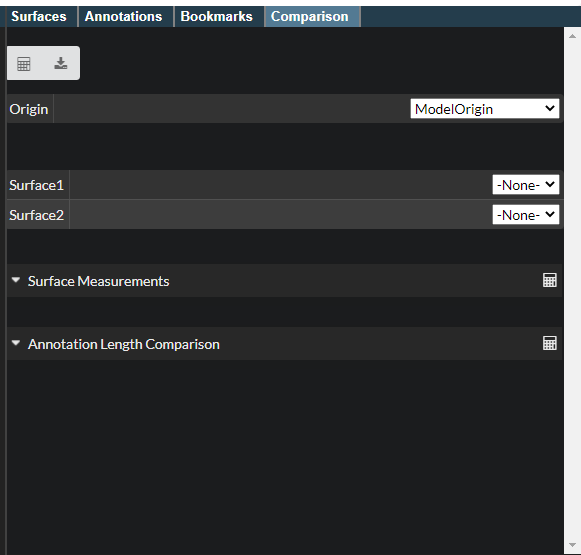
\includegraphics[width=0.6\textwidth]{pics/surfaceComparisonV0.1.PNG}
	\caption[The surface comparison interface.]{The Surface Comparison Interface.}
	\label{fig:surfaceComparison}
\end{figure}

Use the drop down labelled \emph{Origin} to select which point should be used as the centre of a surface for various calculations.

In the drop down boxes labelled \emph{Surface1} and \emph{Surface2} you can select the surfaces you wish to compare. Once you have selected two surfaces, you can toggle their visibility using the \texttt{t} button on your keyboard. The calculation of surface measurements is also triggered by selecting two surfaces. You can update the measurements by clicking on the button with the calculator icon.

To compare length measurements, create a bookmark and make sure it is selected. This bookmark can now be used as a projection point for annotations. For this, select the Bookmark projection mode for annotation drawing (figure \ref{fig:surfaceComparisonBookmarkMode}).

\begin{figure}[h]
	\centering
	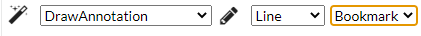
\includegraphics[width=0.7\textwidth]{pics/surfaceComparisonBookmarkMode.PNG}
	\caption[The Bookmark Projection Mode.]{The Bookmark projection mode for comparing length measurements on two surfaces. Make sure a bookmark is selected when using this mode.}
	\label{fig:surfaceComparisonBookmarkMode}
\end{figure}

Now draw one annotation on each of the two surfaces while the same bookmark is selected. Use the \texttt{t} button on your keyboard to toggle visibility between the two surfaces. Return to the comparison window and click the button with the calculator icon to update the calculations. The measurements for annotations are listed under the heading \emph{Annotation Length Comparison}.

To export all measurements click on button with the download icon. The measurements will be saved in the PRo3D home directory. The full path is printed on the console when exporting.

Bookmarks can be exported and imported using the menu. Select the main menu (top left), then \emph{Bookmarks}, then \emph{Import} or \emph{Export}.